\subsection{Control retroalimentado basado en observación}

Considere el sistema SISO
\[(1)
    \left\{
        \begin{array}{lll}
            \dot{x} = Ax + Bu \\
            y = Cx
        \end{array}
    \right.
\]

Teorema 1: si el sistema es estabilizable entonces existe \( k \) tal que la matriz \( A-Bk \) es estable

Teorema 2: si el sistema es detectable entonces existe \( L \) tal que \( A-LC \) es estable

Teorema 3: sea el sistema estabilizable y detectable, entonces existe un observador de estado \( \dot{\hat{x}} = A\hat{x} + Bu + L(y-C\hat{x}) \) y una retroalimentación \( u=r-k\hat{x} \) tal que el sistema acoplado es estable
\begin{figure}[ht]
    \centering
        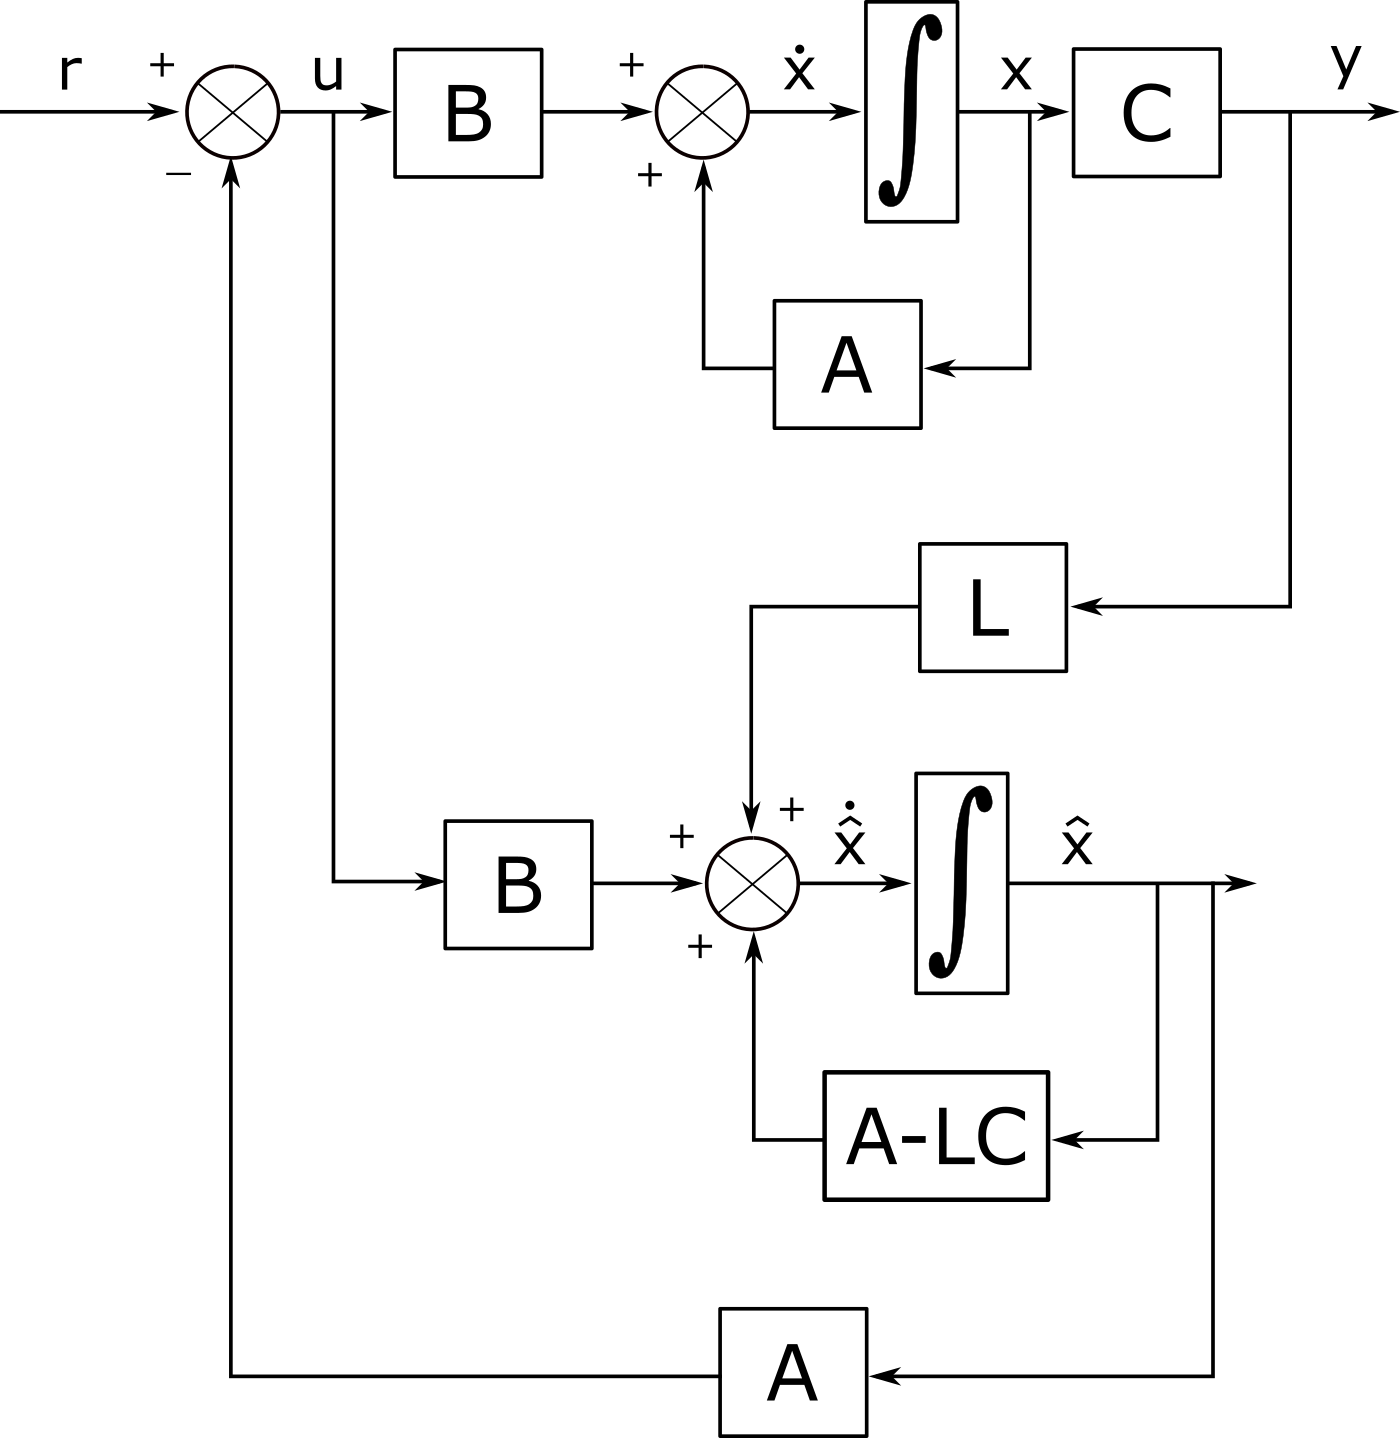
\includegraphics[scale=0.19]{Control de Sistemas Mecatronicos Figuras/11 Sistema con Observador Retroalimentado.png}
        \caption{Sistema retroalimentado basado en observación}
\end{figure}

Sustituyendo la retroalimentación del observador de estado \( u = r-k \hat{x} \) en el sistema (1) y en su observador se tiene que 
\[
    \begin{split}
        \dot{x} & = Ax + B(r-k\hat{x}) \\
        & = Ax - Bk\hat{x} + Br \\ 
        \dot{\hat{x}} & = A\hat{x} + B(r-k\hat{x}) + L(y-C\hat{x}) \\
        & = A\hat{x} - Bk\hat{x} + Br + L(Cx-C\hat{x}) \\
        & = A\hat{x} - Bk\hat{x} + Br + LCx - LC\hat{x} \\
        & = LCx + (A - BK - LC)\hat{x} +Br
    \end{split}
\]

entonces se puede escribir un solo sistema de la siguiente forma
\[
    \begin{bmatrix}
        \dot{x} \\ \dot{\hat{x}}
    \end{bmatrix} =
    \begin{bmatrix}
        A & -Bk \\
        LC & A-Bk-LC 
    \end{bmatrix}
    \begin{bmatrix}
        x \\ \hat{x}
    \end{bmatrix} +
    \begin{bmatrix}
        B \\ B
    \end{bmatrix} r
\]